\documentclass[twocolumn,11pt]{abst}

%\usepackage[dvipdfmx]{subfigure}


% タイトル
\title{安定飛行ができるドローンの開発}

\author{天王地亮太(指導教員 伊藤恒平)}

%\urlstyle{rm}

\setcounter{page}{25}
\lhead{}
\chead{}
\rhead{{\sf 17・213}\\{\bf 機械工学科}}
\lfoot{}
\cfoot{{\sf-\ M-\thepage \ -}}
%\rfoot{}
\renewcommand{\headrulewidth}{3pt}
%\renewcommand{\footrulewidth}{1pt}




\begin{document}
%\layout
\maketitle
\thispagestyle{fancy}
\pagestyle{fancy}

\setlength{\baselineskip}{5.6truemm}
\kanjiskip=.07zw plus 3pt minus 3pt
\xkanjiskip=.07zw plus 3pt minus 3pt


% 本文

\section{緒言}
\subsection{研究の背景}
本年は,自作したドローンで飛行ロボットコンテストという室内飛行機の大会に出場しようと試みた.
飛行ロボットコンテストとは,2006年から開催された日本航空宇宙学会が主催の室内飛行用航空機型ロボットによる競技.自作ドローンが参加可能な,マルチコプタ部門は2015年の第11回から登場した.


\subsection{研究の目的}
ドローンの製作に必要なプログラムと制御に関する知識がなく,結果大会のエントリーの締切までに作り上げることができず,参加すること事態できなかった.そこで製作に関わる制御の知識をドローンを製作しながら学んでいき,ドローンが外部からの突然加わる力によって傾き墜落しないような安定飛行ができる機体の製作を目標とする.


\section{設計製作}
製作するドローンは軽量化をコンセプトとした.
フレームの材料は厚さ2mmのベニヤ板を使用,さらに 図\ref{fig:flame}からわかるに,フレームの所々にトラス構造のような穴をあけ,軽量化とともに剛性も確保した.このフレーム形を手作業で製作するにはかなりの根気や技術,時間を必要とする.この製作をレーザー加工機を使用することによってこの形を綺麗に作るための技術や時間を短縮することに成功した.


\begin{figure}[htbp]
  \begin{center}
    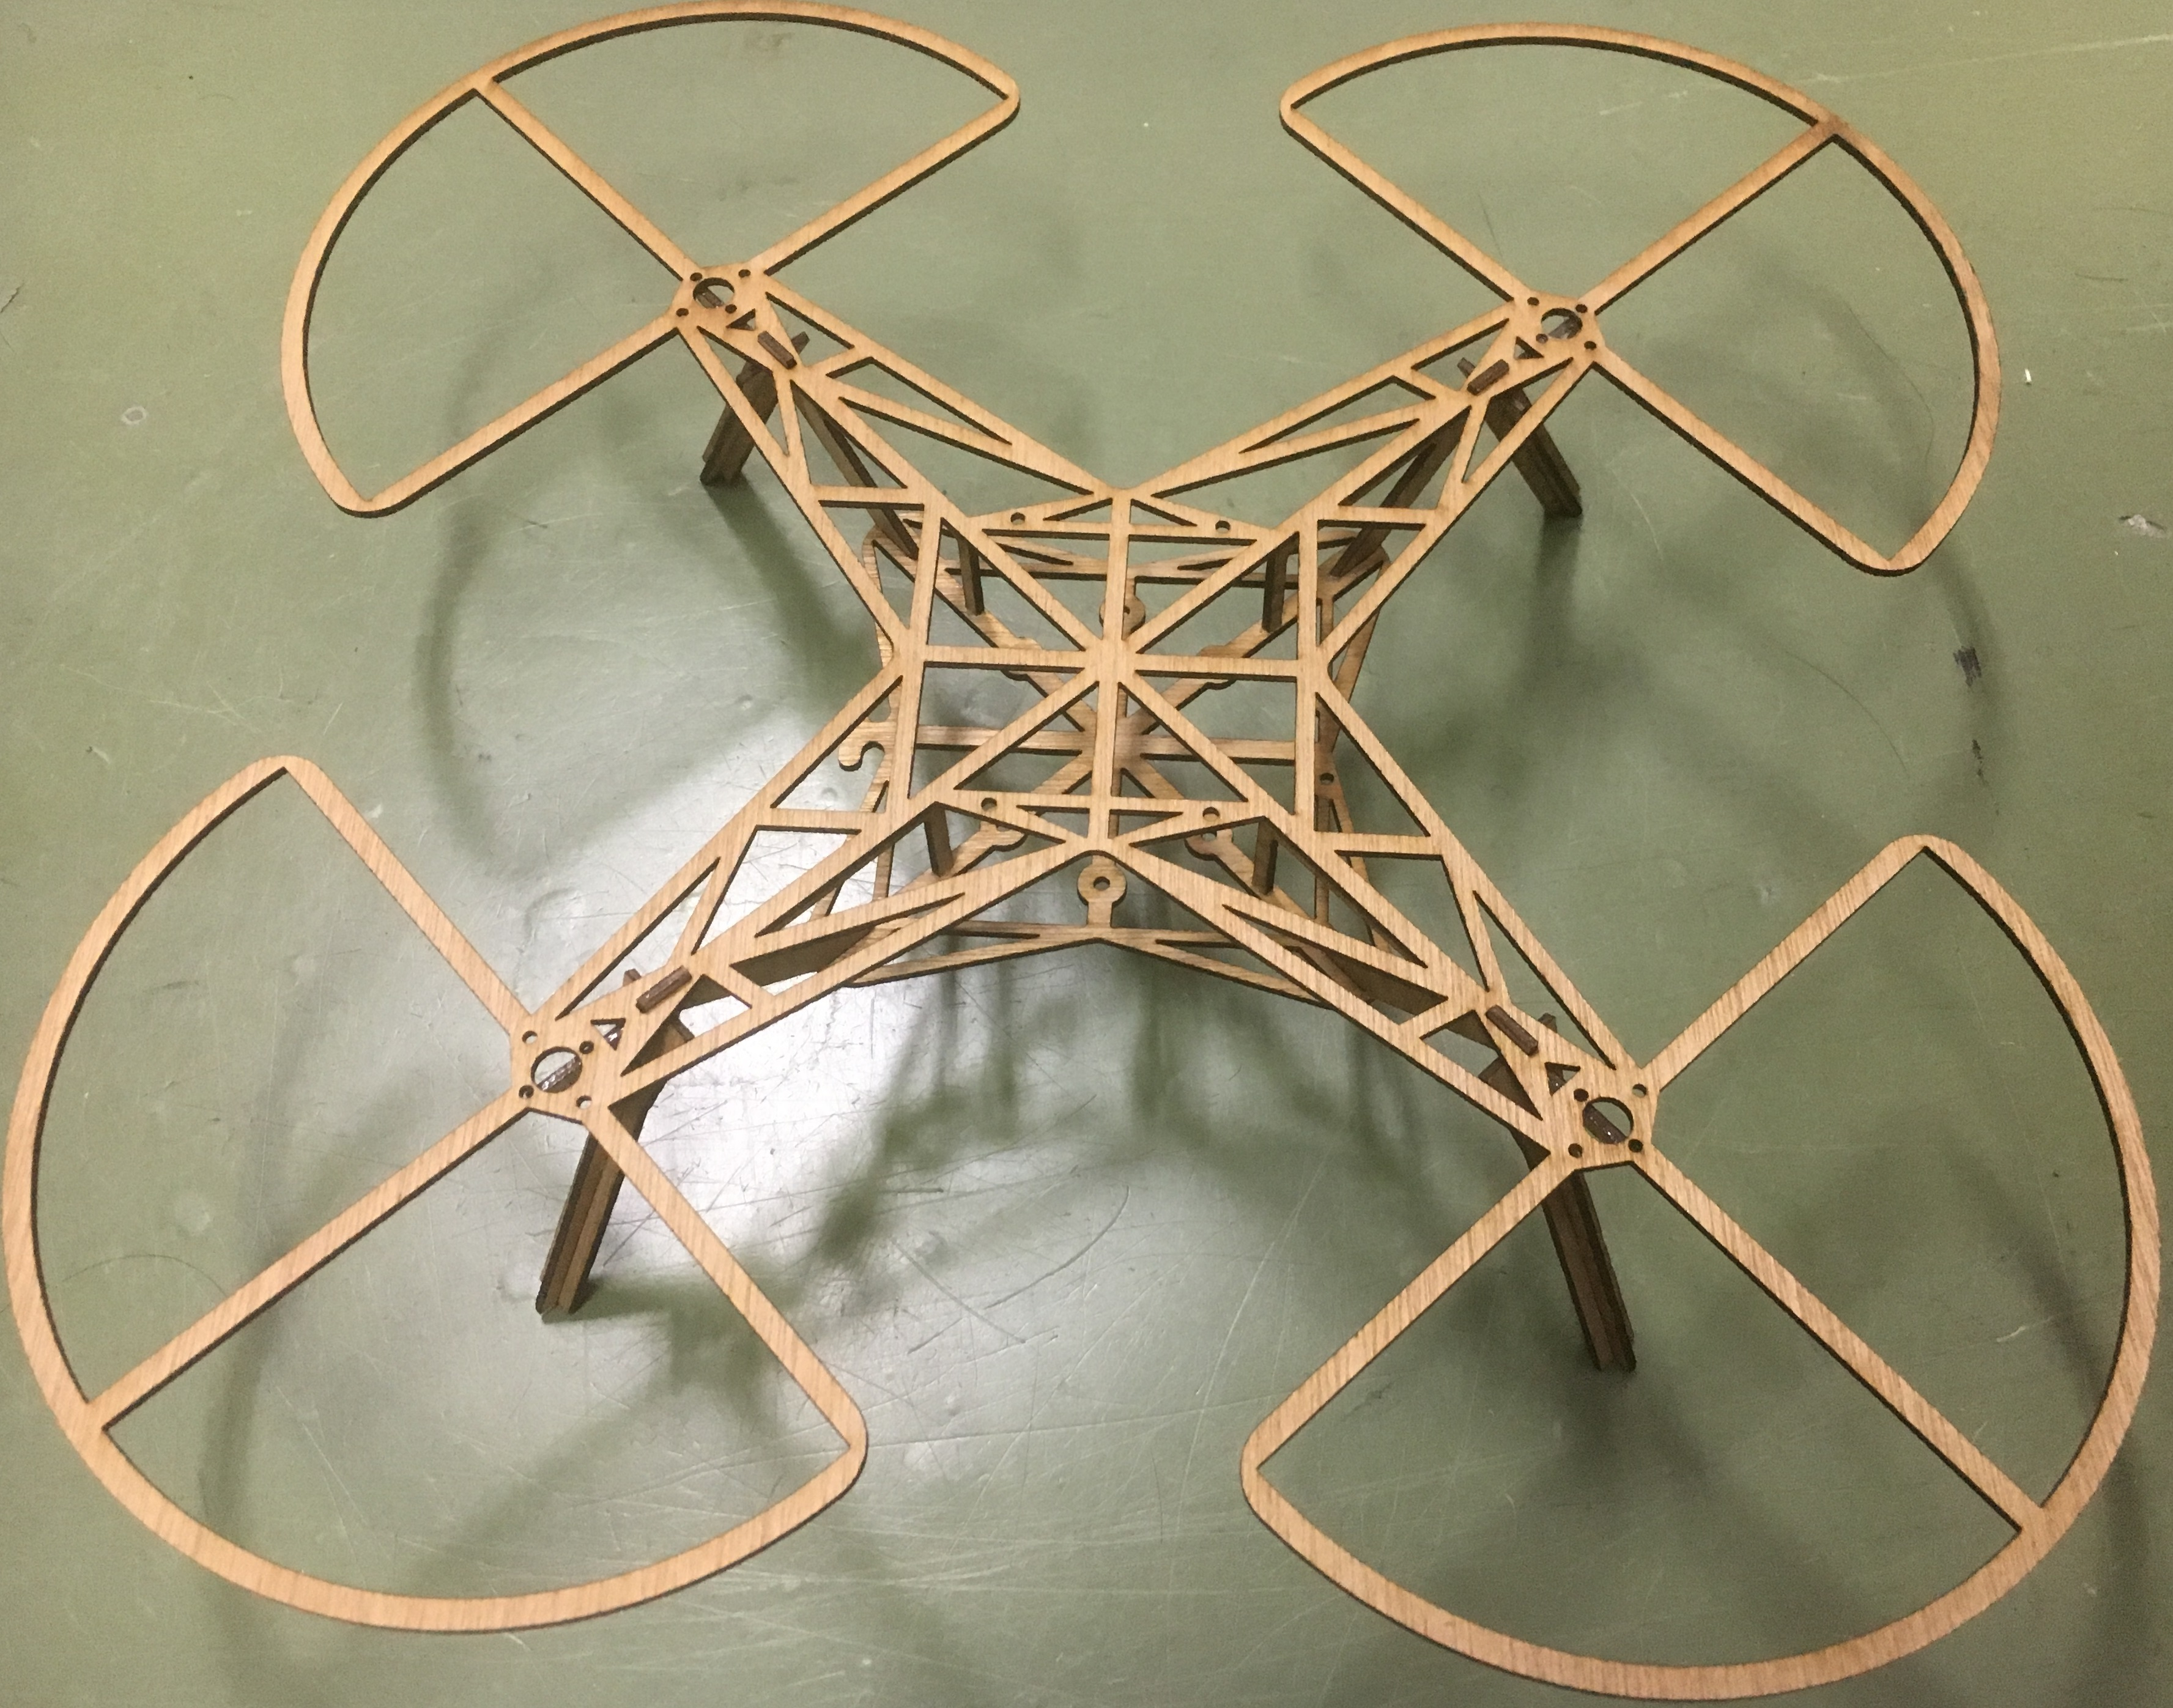
\includegraphics[width=60mm]{flame.jpg}
    \end{center}
  \caption{製作したベニヤフレーム}
 \label{fig:flame}
\end{figure}

\section{ジャイロセンサ}
主に市販で売られているドローンや自作で製作するときに使われているマイコンはフライトコントローラと呼ばれるジャイロセンサ,加速度センサ,気圧センサ,GPSといった機体の姿勢を制御し安定させるセンサを含んだコンピュータを使用しドローンを制御するのだが,今回はマイコンとセンサを別々にし,シリアル通信を利用してセンサから来るデータのやり取りに関する知識を学ぶため,フライトコントローラを使用せずにマイコンとセンサを別々にした.
そして今回の研究で使用するマイコンは秋月電子のRX621で,センサはGY-80というジャイロ,加速度,地磁気といった複数のセンサが一つとなったもの.その中のジャイロセンサだけを使用する.

\begin{figure}[htbp]
  \begin{center}
    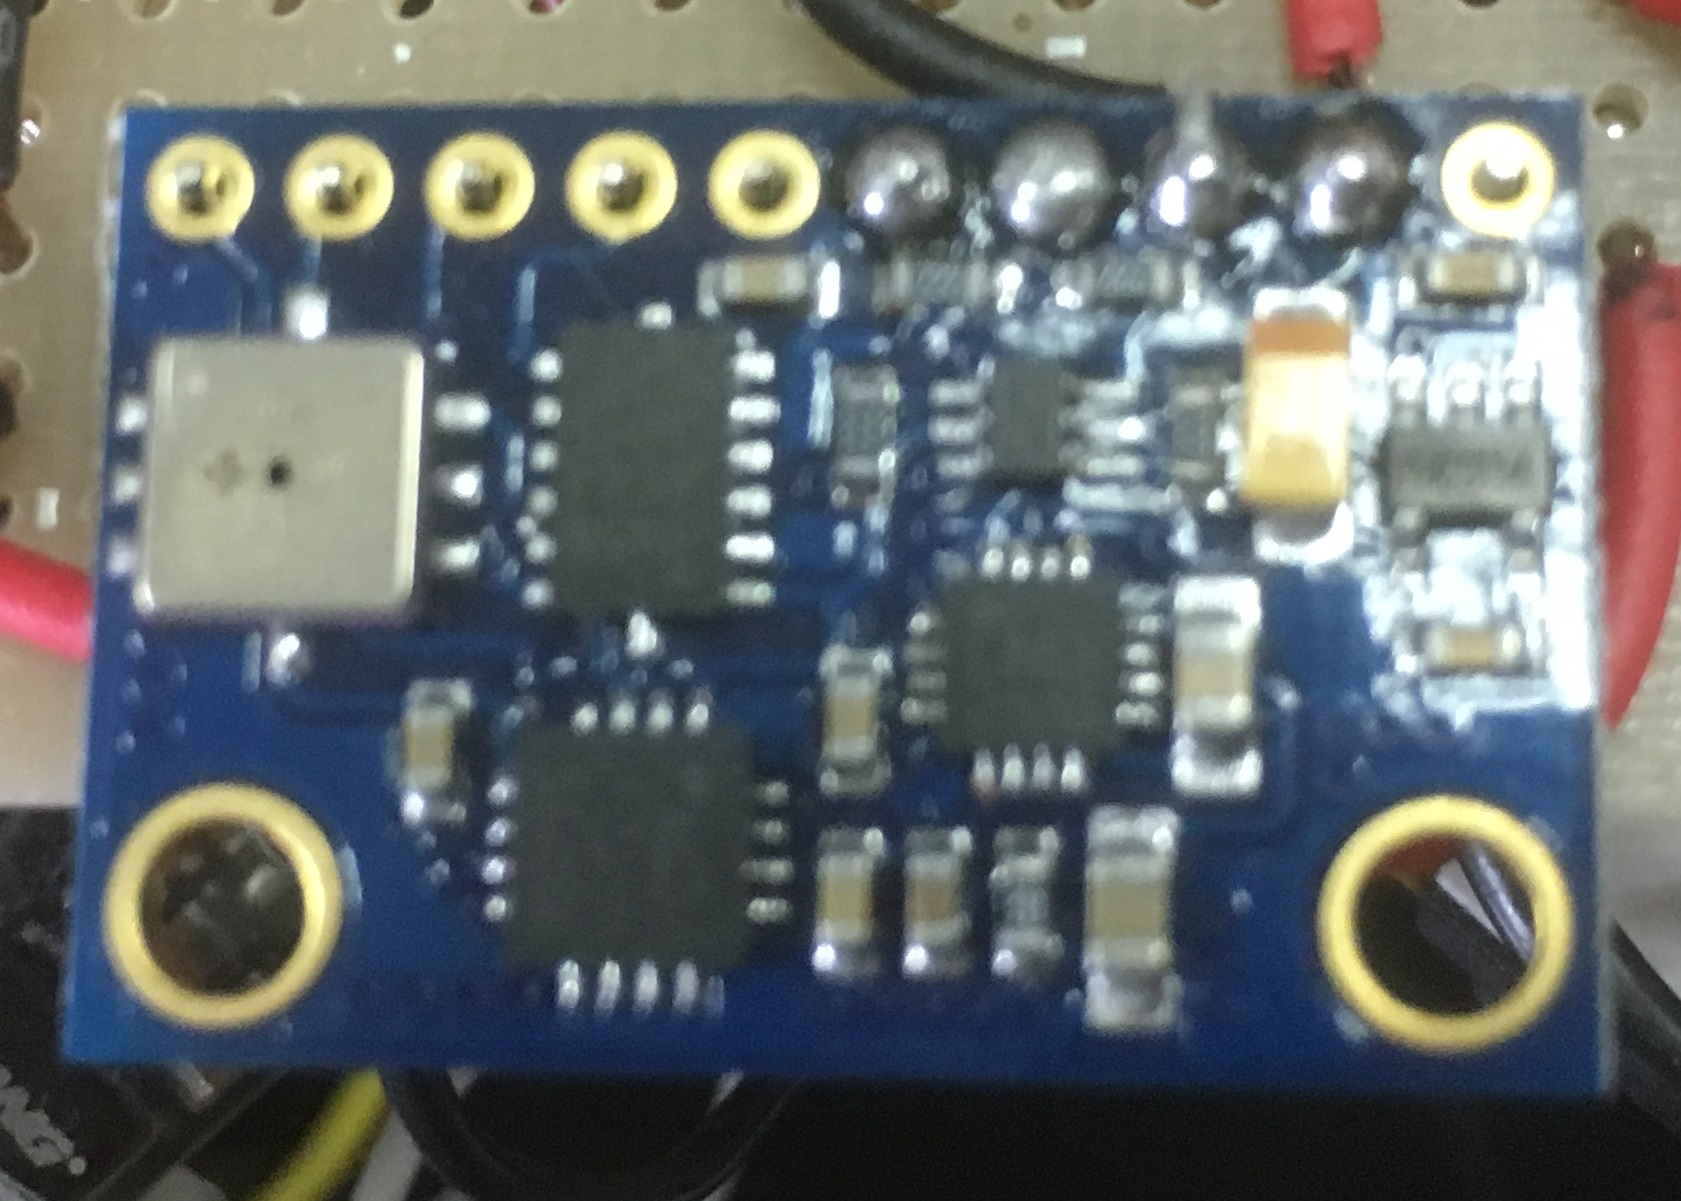
\includegraphics[width=50mm]{GY-80.jpg}
    \end{center}
  \caption{使用するセンサ GY-80}
 \label{fig:GY-80}
\end{figure}


\subsection{I2C通信}
このジャイロセンサとマイコンとのデータのやり取りはI2C通信を使用しデータ通信を行う.

I2C(Inter-Integrated Circuit)とは,フィリップス社が開発した複数のデバイスとシリアル通信を行う通信方法の1つである.
この通信方法の大きな特徴はデータ通信のすべての権限を持つデバイス(マスタ)とそれ以外のデバイス(スレーブ)間で2本の信号線SDA(シリアルデータ)とSCL(シリアルクロック)でマスタとスレーブ間のデータ通信を行う.ここでのマスタ側のデバイスはマイコンで,スレーブ側をジャイロセンサとする.この関係図を図 \ref{fig:i2c} に示す.

\begin{figure}[htbp]
  \begin{center}
    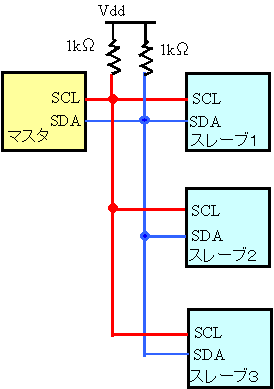
\includegraphics[width=30mm]{i2c.png}
    \end{center}
  \caption{I2C通信}
 \label{fig:i2c}
\end{figure}

\subsection{プログラム製作}

\subsubsection{SCLとSDA}
図 \ref{fig:i2c}にあるSCLはスレーブとの同期をとるための信号線で,通常はマスターからスレーブへの一方通行の線である.
一方,SDAはSCLに同期し,データの転送に用いる信号線であり,マスターとスレーブ,どちらからも送信される.

\subsubsection{書込みの流れ}

マスタ側からスタートコンディションを発行し通信を開始したら,マスタ側から''通信するスレーブ''と''マスタ側が書込み''アドレスを8bit分送信しスレーブ側から正常に送信されたことを意味するACKという1bit分のデータが返される.この次からスレーブに書き込みたいデータを約1byte分送りACKがスレーブから送られる.そしてすべてのデータの送信が終了したら,ストップコンディションを発行し通信を終える.

\begin{figure}[htbp]
  \begin{center}
    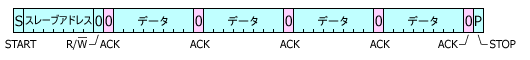
\includegraphics[width=60mm]{i2c_w.png}
    \end{center}
  \caption{I2C書込み}
 \label{fig:i2c_w}
\end{figure}

\subsubsection{読込みの流れ}

マスタ側からスタートコンディションを発行し通信を開始したら,マスタ側から''通信するスレーブ''と''マスタ側が読込む''アドレスを8bit分送信しスレーブ側からACKが返される.そしてスレーブから送られるデータを約1byte分もらい,ACKをスレーブに送る.そしてすべてのデータの送信が終了したら,ストップコンディションを発行し通信を終える.

\begin{figure}[htbp]
  \begin{center}
    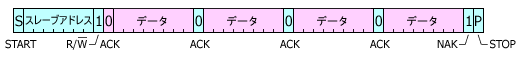
\includegraphics[width=60mm]{i2c_r.png}
    \end{center}
  \caption{I2C読込み}
 \label{fig:i2c_r}
\end{figure}

\subsection{データ取得}
通信で得たデータは,図\ref{fig:roll}より10000近くのデータを取得しそのデータを平均した値を,制御に反映させるデータから引く動作が必要となる.これをキャリブレーションという.こうして得た値を台形法の積分方法を用いることで角度を求めるため値が図\ref{fig:roll_deg}となっている.
しかし,図\ref{fig:roll}と図\ref{fig:roll_deg}の縦軸のデータの値は通信用のデータであって本当の角速度や角度ではない.
そのためセンサを90度傾け,この時の値で90を割るように計算することで1度傾いた時の値を調べる必要がある.

\begin{figure}[htbp]
  \begin{center}
    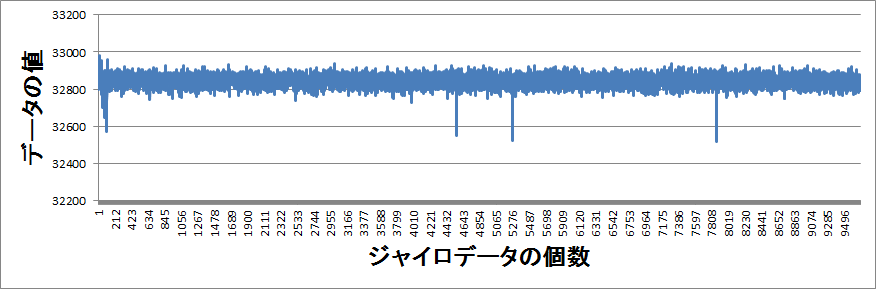
\includegraphics[width=65mm]{roll.png}
    \end{center}
  \caption{キャリブレーション用データ}
 \label{fig:roll}
\end{figure}

\begin{figure}[htbp]
  \begin{center}
    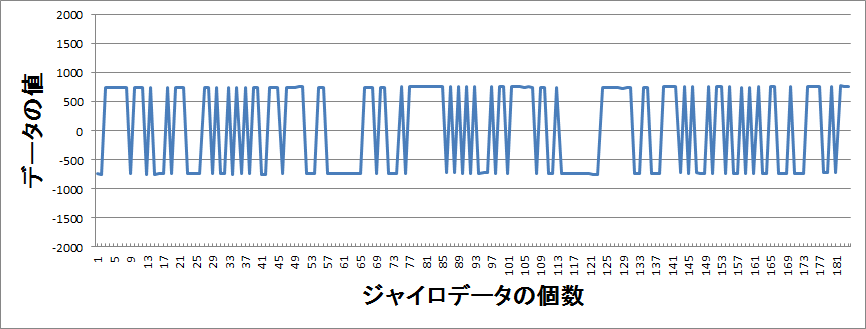
\includegraphics[width=65mm]{roll_deg.png}
    \end{center}
  \caption{台形積分で求めたのロールデータ}
 \label{fig:roll_deg}
\end{figure}

\section{結言}
データの取得及び処理まで至れたが,今だドローンを飛ばすまでには到達できていない.しかし,後は各ドローンの制御プログラムを合わせ,ジャイロセンサの値でモーターを制御するというところまで到達しているため,今後この製作をしていく予定である.

% 参考文献
\begin{thebibliography}{8}
\bibitem{maikon} 新海栄治,石黒裕紀,伊藤彩子, 仲めぐみ,藤澤幸穂:RXマイコンのすべて,株式会社 電波新聞社,2012
\bibitem{i2c} I2C通信の使い方-電子工作の実験室,http://www.picfun.com/c15.html , 
\end{thebibliography}



\end{document}

○○○○○○○○○○○○○○○○○○○○○○○○○○○○○○○○○○○○○○○○○○○○○○○○
○○○○○○○○○○○○○○○○○○○○○○○○○○○○○○○○○○○○○○○○○○○○○○○○
○○○○○○○○○○○○○○○○○○○○○○○○○○○○○○○○○○○○○○○○○○○○○○○○
○○○○○○○○○○○○○○○○○○○○○○○○○○○○○○○○○○○○○○○○○○○○○○○○
○○○○○○○○○○○○○○○○○○○○○○○○○○○○○○○○○○○○○○○○○○○○○○○○
○○○○○○○○○○○○○○○○○○○○○○○○○○○○○○○○○○○○○○○○○○○○○○○○
○○○○○○○○○○○○○○○○○○○○○○○○○○○○○○○○○○○○○○○○○○○○○○○○
○○○○○○○○○○○○○○○○○○○○○○○○○○○○○○○○○○○○○○○○○○○○○○○○
○○○○○○○○○○○○○○○○○○○○○○○○○○○○○○○○○○○○○○○○○○○○○○○○
○○○○○○○○○○○○○○○○○○○○○○○○○○○○○○○○○○○○○○○○○○○○○○○○
○○○○○○○○○○○○○○○○○○○○○○○○○○○○○○○○○○○○○○○○○○○○○○○○
○○○○○○○○○○○○○○○○○○○○○○○○○○○○○○○○○○○○○○○○○○○○○○○○
○○○○○○○○○○○○○○○○○○○○○○○○○○○○○○○○○○○○○○○○○○○○○○○○
○○○○○○○○○○○○○○○○○○○○○○○○○○○○○○○○○○○○○○○○○○○○○○○○
○○○○○○○○○○○○○○○○○○○○○○○○○○○○○○○○○○○○○○○○○○○○○○○○
○○○○○○○○○○○○○○○○○○○○○○○○○○○○○○○○○○○○○○○○○○○○○○○○
○○○○○○○○○○○○○○○○○○○○○○○○○○○○○○○○○○○○○○○○○○○○○○○○
○○○○○○○○○○○○○○○○○○○○○○○○○○○○○○○○○○○○○○○○○○○○○○○○
○○○○○○○○○○○○○○○○○○○○○○○○○○○○○○○○○○○○○○○○○○○○○○○○
○○○○○○○○○○○○○○○○○○○○○○○○○○○○○○○○○○○○○○○○○○○○○○○○
○○○○○○○○○○○○○○○○○○○○○○○○○○○○○○○○○○○○○○○○○○○○○○○○
○○○○○○○○○○○○○○○○○○○○○○○○○○○○○○○○○○○○○○○○○○○○○○○○
○○○○○○○○○○○○○○○○○○○○○○○○○○○○○○○○○○○○○○○○○○○○○○○○
○○○○○○○○○○○○○○○○○○○○○○○○○○○○○○○○○○○○○○○○○○○○○○○○
○○○○○○○○○○○○○○○○○○○○○○○○○○○○○○○○○○○○○○○○○○○○○○○○
○○○○○○○○○○○○○○○○○○○○○○○○○○○○○○○○○○○○○○○○○○○○○○○○
○○○○○○○○○○○○○○○○○○○○○○○○○○○○○○○○○○○○○○○○○○○○○○○○
○○○○○○○○○○○○○○○○○○○○○○○○○○○○○○○○○○○○○○○○○○○○○○○○
○○○○○○○○○○○○○○○○○○○○○○○○○○○○○○○○○○○○○○○○○○○○○○○○
○○○○○○○○○○○○○○○○○○○○○○○○○○○○○○○○○○○○○○○○○○○○○○○○
○○○○○○○○○○○○○○○○○○○○○○○○○○○○○○○○○○○○○○○○○○○○○○○○
○○○○○○○○○○○○○○○○○○○○○○○○○○○○○○○○○○○○○○○○○○○○○○○○
○○○○○○○○○○○○○○○○○○○○○○○○○○○○○○○○○○○○○○○○○○○○○○○○
○○○○○○○○○○○○○○○○○○○○○○○○○○○○○○○○○○○○○○○○○○○○○○○○
○○○○○○○○○○○○○○○○○○○○○○○○○○○○○○○○○○○○○○○○○○○○○○○○
○○○○○○○○○○○○○○○○○○○○○○○○○○○○○○○○○○○○○○○○○○○○○○○○
○○○○○○○○○○○○○○○○○○○○○○○○○○○○○○○○○○○○○○○○○○○○○○○○
○○○○○○○○○○○○○○○○○○○○○○○○○○○○○○○○○○○○○○○○○○○○○○○○
○○○○○○○○○○○○○○○○○○○○○○○○○○○○○○○○○○○○○○○○○○○○○○○○
○○○○○○○○○○○○○○○○○○○○○○○○○○○○○○○○○○○○○○○○○○○○○○○○
○○○○○○○○○○○○○○○○○○○○○○○○○○○○○○○○○○○○○○○○○○○○○○○○
○○○○○○○○○○○○○○○○○○○○○○○○○○○○○○○○○○○○○○○○○○○○○○○○
○○○○○○○○○○○○○○○○○○○○○○○○○○○○○○○○○○○○○○○○○○○○○○○○
○○○○○○○○○○○○○○○○○○○○○○○○○○○○○○○○○○○○○○○○○○○○○○○○
○○○○○○○○○○○○○○○○○○○○○○○○○○○○○○○○○○○○○○○○○○○○○○○○
○○○○○○○○○○○○○○○○○○○○○○○○○○○○○○○○○○○○○○○○○○○○○○○○
○○○○○○○○○○○○○○○○○○○○○○○○○○○○○○○○○○○○○○○○○○○○○○○○
○○○○○○○○○○○○○○○○○○○○○○○○○○○○○○○○○○○○○○○○○○○○○○○○
○○○○○○○○○○○○○○○○○○○○○○○○○○○○○○○○○○○○○○○○○○○○○○○○
○○○○○○○○○○○○○○○○○○○○○○○○○○○○○○○○○○○○○○○○○○○○○○○○
○○○○○○○○○○○○○○○○○○○○○○○○○○○○○○○○○○○○○○○○○○○○○○○○
○○○○○○○○○○○○○○○○○○○○○○○○○○○○○○○○○○○○○○○○○○○○○○○○
○○○○○○○○○○○○○○○○○○○○○○○○○○○○○○○○○○○○○○○○○○○○○○○○
○○○○○○○○○○○○○○○○○○○○○○○○○○○○○○○○○○○○○○○○○○○○○○○○
○○○○○○○○○○○○○○○○○○○○○○○○○○○○○○○○○○○○○○○○○○○○○○○○
○○○○○○○○○○○○○○○○○○○○○○○○○○○○○○○○○○○○○○○○○○○○○○○○
○○○○○○○○○○○○○○○○○○○○○○○○○○○○○○○○○○○○○○○○○○○○○○○○
○○○○○○○○○○○○○○○○○○○○○○○○○○○○○○○○○○○○○○○○○○○○○○○○
○○○○○○○○○○○○○○○○○○○○○○○○○○○○○○○○○○○○○○○○○○○○○○○○
○○○○○○○○○○○○○○○○○○○○○○○○○○○○○○○○○○○○○○○○○○○○○○○○
○○○○○○○○○○○○○○○○○○○○○○○○○○○○○○○○○○○○○○○○○○○○○○○○
○○○○○○○○○○○○○○○○○○○○○○○○○○○○○○○○○○○○○○○○○○○○○○○○
○○○○○○○○○○○○○○○○○○○○○○○○○○○○○○○○○○○○○○○○○○○○○○○○
○○○○○○○○○○○○○○○○○○○○○○○○○○○○○○○○○○○○○○○○○○○○○○○○
○○○○○○○○○○○○○○○○○○○○○○○○○○○○○○○○○○○○○○○○○○○○○○○○
○○○○○○○○○○○○○○○○○○○○○○○○○○○○○○○○○○○○○○○○○○○○○○○○
○○○○○○○○○○○○○○○○○○○○○○○○○○○○○○○○○○○○○○○○○○○○○○○○
○○○○○○○○○○○○○○○○○○○○○○○○○○○○○○○○○○○○○○○○○○○○○○○○
○○○○○○○○○○○○○○○○○○○○○○○○○○○○○○○○○○○○○○○○○○○○○○○○
○○○○○○○○○○○○○○○○○○○○○○○○○○○○○○○○○○○○○○○○○○○○○○○○
○○○○○○○○○○○○○○○○○○○○○○○○○○○○○○○○○○○○○○○○○○○○○○○○
○○○○○○○○○○○○○○○○○○○○○○○○○○○○○○○○○○○○○○○○○○○○○○○○
○○○○○○○○○○○○○○○○○○○○○○○○○○○○○○○○○○○○○○○○○○○○○○○○
○○○○○○○○○○○○○○○○○○○○○○○○○○○○○○○○○○○○○○○○○○○○○○○○
○○○○○○○○○○○○○○○○○○○○○○○○○○○○○○○○○○○○○○○○○○○○○○○○
○○○○○○○○○○○○○○○○○○○○○○○○○○○○○○○○○○○○○○○○○○○○○○○○
○○○○○○○○○○○○○○○○○○○○○○○○○○○○○○○○○○○○○○○○○○○○○○○○
○○○○○○○○○○○○○○○○○○○○○○○○○○○○○○○○○○○○○○○○○○○○○○○○
○○○○○○○○○○○○○○○○○○○○○○○○○○○○○○○○○○○○○○○○○○○○○○○○
○○○○○○○○○○○○○○○○○○○○○○○○○○○○○○○○○○○○○○○○○○○○○○○○
○○○○○○○○○○○○○○○○○○○○○○○○○○○○○○○○○○○○○○○○○○○○○○○○
○○○○○○○○○○○○○○○○○○○○○○○○○○○○○○○○○○○○○○○○○○○○○○○○
○○○○○○○○○○○○○○○○○○○○○○○○○○○○○○○○○○○○○○○○○○○○○○○○
○○○○○○○○○○○○○○○○○○○○○○○○○○○○○○○○○○○○○○○○○○○○○○○○
○○○○○○○○○○○○○○○○○○○○○○○○○○○○○○○○○○○○○○○○○○○○○○○○
○○○○○○○○○○○○○○○○○○○○○○○○○○○○○○○○○○○○○○○○○○○○○○○○
○○○○○○○○○○○○○○○○○○○○○○○○○○○○○○○○○○○○○○○○○○○○○○○○
○○○○○○○○○○○○○○○○○○○○○○○○○○○○○○○○○○○○○○○○○○○○○○○○
○○○○○○○○○○○○○○○○○○○○○○○○○○○○○○○○○○○○○○○○○○○○○○○○
○○○○○○○○○○○○○○○○○○○○○○○○○○○○○○○○○○○○○○○○○○○○○○○○
○○○○○○○○○○○○○○○○○○○○○○○○○○○○○○○○○○○○○○○○○○○○○○○○
○○○○○○○○○○○○○○○○○○○○○○○○○○○○○○○○○○○○○○○○○○○○○○○○
○○○○○○○○○○○○○○○○○○○○○○○○○○○○○○○○○○○○○○○○○○○○○○○○
○○○○○○○○○○○○○○○○○○○○○○○○○○○○○○○○○○○○○○○○○○○○○○○○
○○○○○○○○○○○○○○○○○○○○○○○○○○○○○○○○○○○○○○○○○○○○○○○○
○○○○○○○○○○○○○○○○○○○○○○○○○○○○○○○○○○○○○○○○○○○○○○○○
○○○○○○○○○○○○○○○○○○○○○○○○○○○○○○○○○○○○○○○○○○○○○○○○
○○○○○○○○○○○○○○○○○○○○○○○○○○○○○○○○○○○○○○○○○○○○○○○○
○○○○○○○○○○○○○○○○○○○○○○○○○○○○○○○○○○○○○○○○○○○○○○○○
○○○○○○○○○○○○○○○○○○○○○○○○○○○○○○○○○○○○○○○○○○○○○○○○
○○○○○○○○○○○○○○○○○○○○○○○○○○○○○○○○○○○○○○○○○○○○○○○○
○○○○○○○○○○○○○○○○○○○○○○○○○○○○○○○○○○○○○○○○○○○○○○○○
○○○○○○○○○○○○○○○○○○○○○○○○○○○○○○○○○○○○○○○○○○○○○○○○
○○○○○○○○○○○○○○○○○○○○○○○○○○○○○○○○○○○○○○○○○○○○○○○○


